% Sections 10-12: Experimental Setup, Results, Performance Analysis. Shared by both templates.

\section{Experimental Setup}\label{sec:setup}

\subsection{Platforms}
No single machine available to the team had both a GPU and many CPU cores, so experiments ran on
two platforms (Table~\ref{tab:platforms}): GPU experiments on a Google Colab Tesla T4 (which has
only 2 CPU threads), and CPU scaling experiments on a 16-thread laptop. A 4-core Linux machine
was used for the live demo run and its screenshot.

\begin{table}[t]
\centering
\caption{Experimental platforms and software.}
\label{tab:platforms}
\footnotesize
\begin{tabularx}{\columnwidth}{@{}l X X@{}}
\toprule
 & GPU platform & CPU platform\\
\midrule
Machine & Google Colab VM & laptop, Windows + WSL2\\
CPU & 2 vCPU (Intel Xeon) & 16 threads (Intel, Iris Xe graphics)\\
GPU & NVIDIA Tesla T4 (Turing, sm\_75), 2560 cores, 16\,GB, 320\,GB/s & none\\
OS & Ubuntu 24.04 & Ubuntu 24.04 (WSL2)\\
Compiler & g++ 13.3, nvcc 13.0, \texttt{-O3 -march=native} & g++, \texttt{-O3 -march=native}\\
MPI & Open MPI 4.1.6 & Open MPI\\
Profilers & Nsight Systems / Compute 2025.3 & built-in phase timers\\
Used for & objectives 3, 6, 8; determinism & objectives 4, 5, 7; determinism\\
\bottomrule
\end{tabularx}
\end{table}

\subsection{Workloads and parameters}
Unless stated otherwise, runs use the default agent mix (Table~\ref{tab:agents}), 4096 price
levels per instrument, an order lifetime of 100 ticks, and seed 42. The experiment sets were:
\begin{itemize}
\item \textbf{Determinism:} 50{,}000 agents, 16 instruments, 500 ticks, seed 1234, on 12 back-end
  configurations (Colab) and on serial, OpenMP 1--16 threads and MPI 1/2/4 ranks with 400{,}000
  agents and 64 instruments (laptop).
\item \textbf{CPU vs GPU crossover:} 1k to 2M agents, 128 instruments, 200 ticks.
\item \textbf{Kernel experiments:} 1M agents, 128 instruments; block size 32--1024; type sorting
  and compaction on/off; Nsight Compute on one tick.
\item \textbf{Agents at fixed instruments (Gustafson):} 32 instruments, 32k to 2M agents.
\item \textbf{Instruments sweep:} 200{,}000 agents, 16 threads, 1 to 128 instruments, serial vs
  OpenMP matching.
\item \textbf{Strong scaling:} 400{,}000 agents, 64 instruments, 300 ticks, 1 to 16 threads.
\item \textbf{Weak scaling:} 50{,}000 agents and 8 instruments per thread, 300 ticks.
\item \textbf{MPI:} 400{,}000 agents, 64 instruments, 1, 2 and 4 ranks (16 threads in total).
\item \textbf{False sharing:} padded vs unpadded per-thread counters, 200{,}000 agents,
  256 instruments, 16 threads.
\item \textbf{Stylised facts:} 64{,}000 agents, 16 instruments, 20{,}000 ticks.
\end{itemize}

\subsection{Methodology}
Each configuration ran 3 times (Colab, first laptop run) or 5 times (laptop strong and weak
scaling), and we report the median. For strong and weak scaling the configurations were
\emph{interleaved} (one run of each configuration per round), with the laptop plugged in and set to
its best-performance power mode; a first, non-interleaved run was discarded because the serial
and 1-thread OpenMP times differed by 60\% under identical work. All raw CSV files are in the
repository's \texttt{results/} folder, and every experiment is reproducible with
\texttt{scripts/bench.sh}.

\section{Results}\label{sec:results}

\subsection{Correctness and execution}\label{sec:res-correct}
All 259{,}597 unit-test checks pass, including a randomised test that compares the order book
against a simple reference implementation and tests that compare each parallel back end against
the serial one (Fig.~\ref{fig:exec-tests}). On the T4, all 12 configurations (serial; OpenMP with
1, 2, 4 and 8 threads; CUDA with and without sorting and compaction; MPI with 2 and 4 ranks using
OpenMP and CUDA) produced the identical trade log: 1{,}289{,}848 trades with fingerprint
\texttt{2b39a9b633ea375b} (Fig.~\ref{fig:exec-det}). On the laptop, serial, OpenMP with 1 to 16
threads and MPI with 1, 2 and 4 ranks all gave fingerprint \texttt{cd3e16901eff5bb0} for
5{,}013{,}234 trades. Fig.~\ref{fig:exec-demo} shows the live demonstration script: the input is
the command line (agents, instruments, ticks, seed) and the output is the number of trades, the
fingerprint and the time per back end. Fig.~\ref{fig:exec-env} shows the GPU environment check.

\begin{figure}[t]
\centering
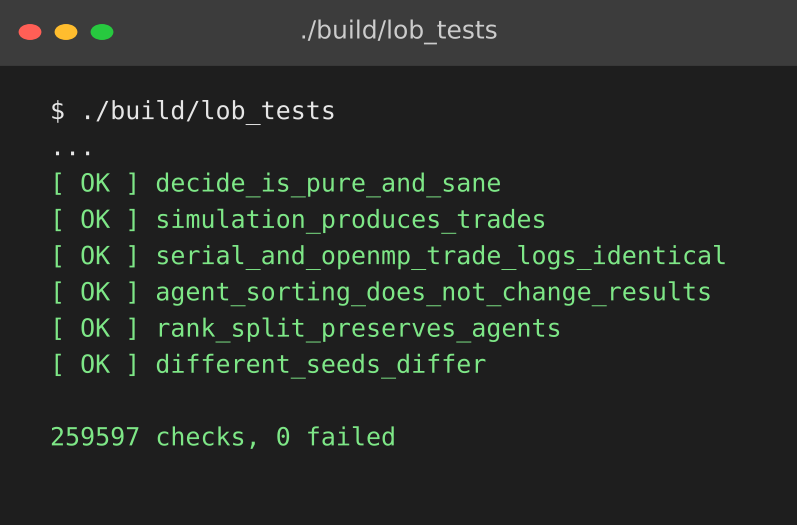
\includegraphics[width=0.8\columnwidth]{exec_tests.png}
\caption{Execution: unit test run (end of output).}
\label{fig:exec-tests}
\end{figure}

\begin{figure}[t]
\centering
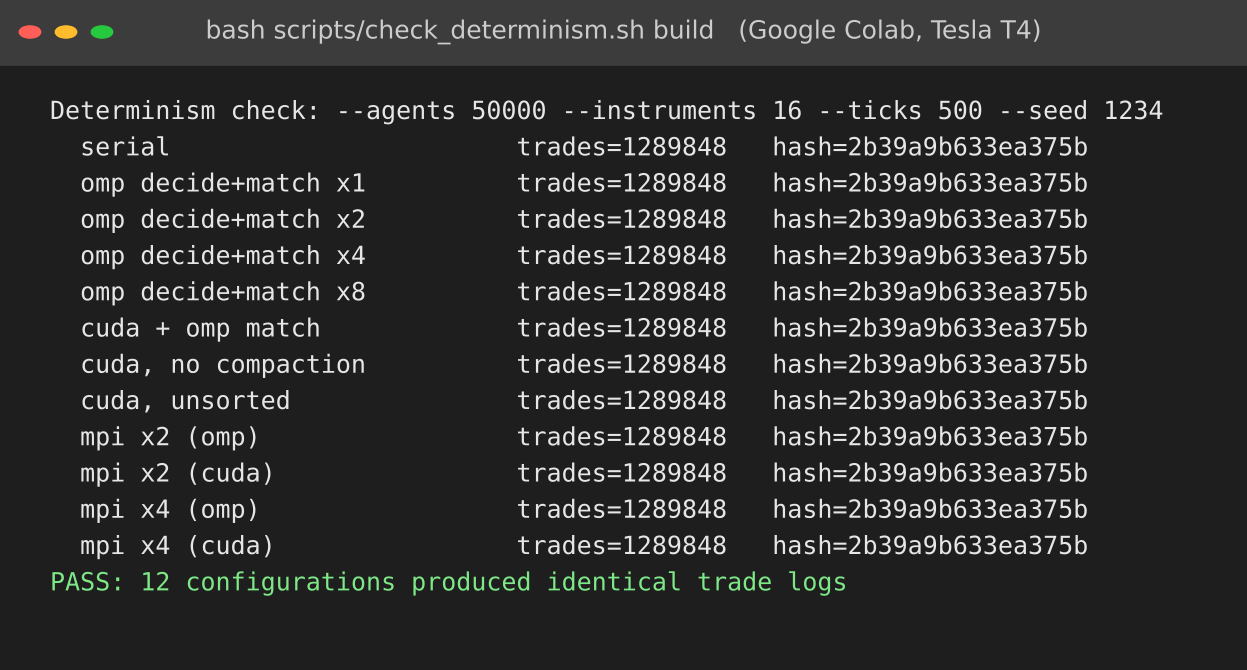
\includegraphics[width=\columnwidth]{exec_determinism_colab.png}
\caption{Execution on the Tesla T4: determinism check across 12 back-end configurations (output of
\texttt{scripts/check\_determinism.sh}).}
\label{fig:exec-det}
\end{figure}

\begin{figure}[t]
\centering
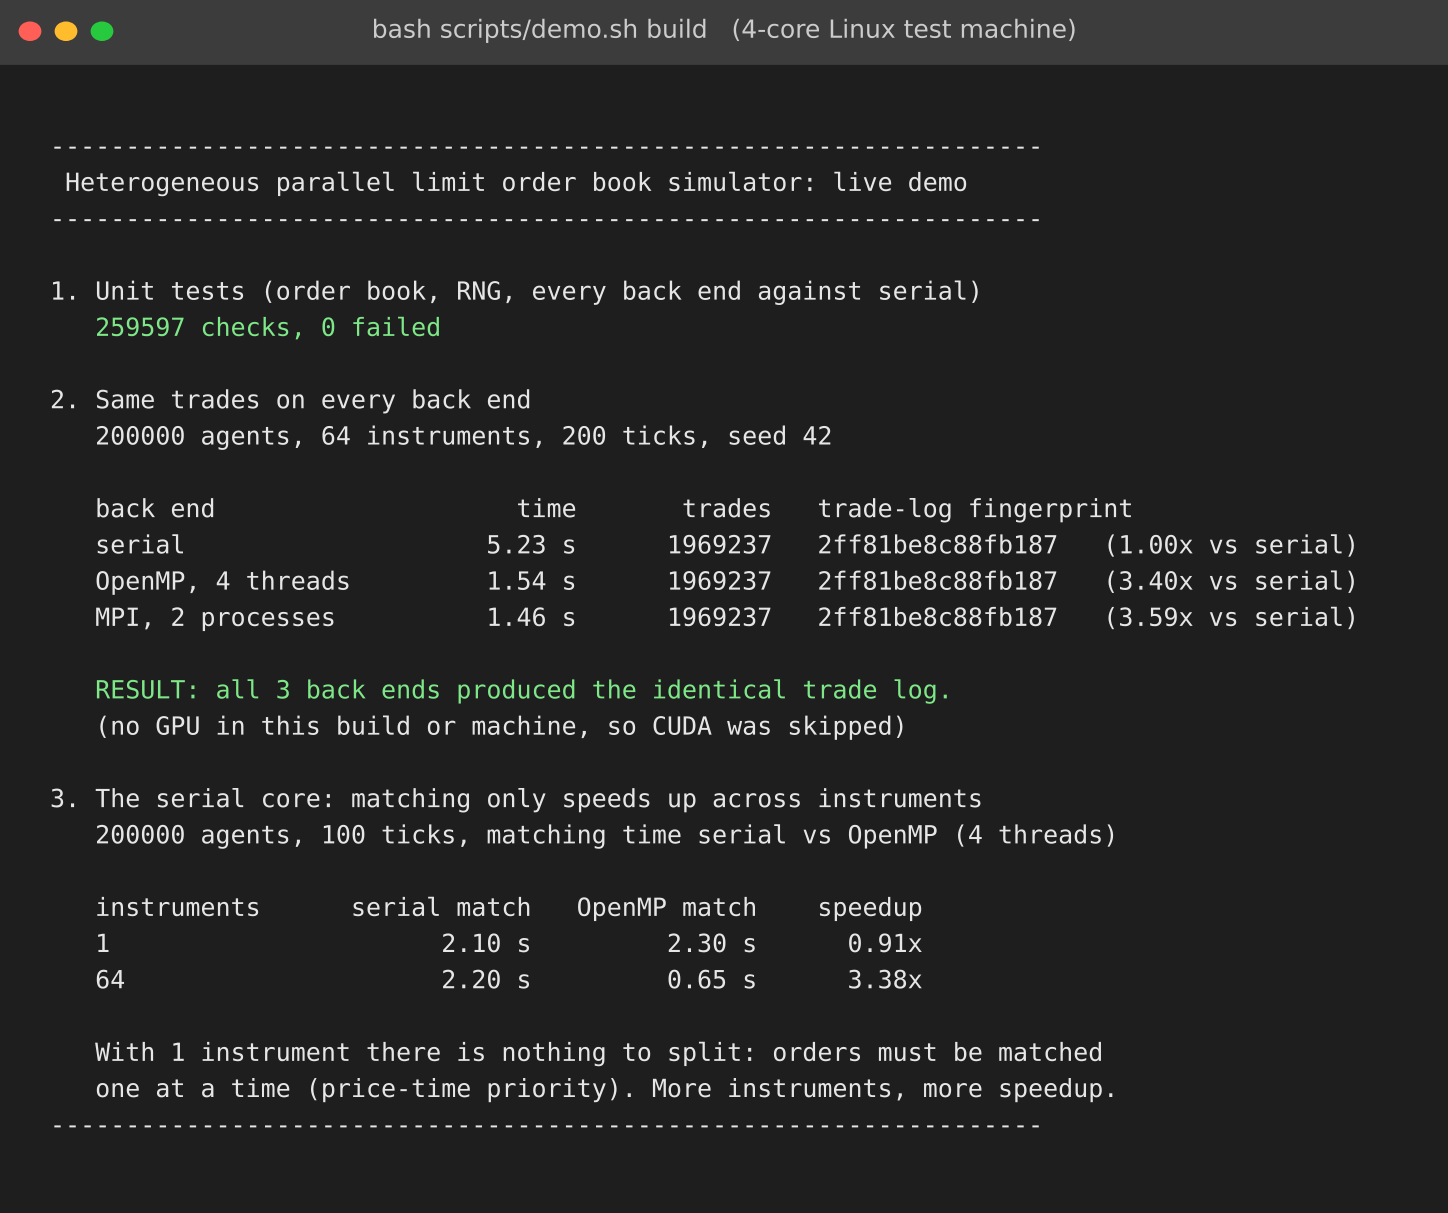
\includegraphics[width=\columnwidth]{exec_demo.png}
\caption{Execution: the live demo (\texttt{bash scripts/demo.sh build}) on a 4-core Linux machine
with 200{,}000 agents, 64 instruments and 200 ticks. Serial, OpenMP and MPI produce the same
1{,}969{,}237 trades and fingerprint; the last table shows that matching speeds up with 64
instruments but not with one.}
\label{fig:exec-demo}
\end{figure}

\begin{figure}[t]
\centering
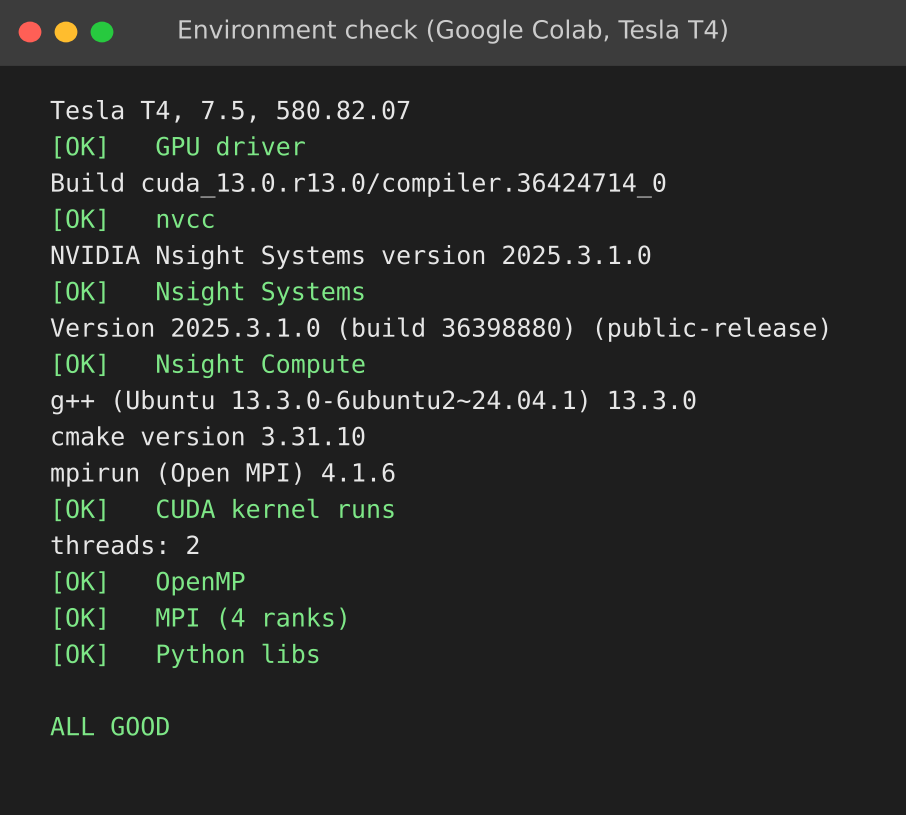
\includegraphics[width=0.75\columnwidth]{exec_colab_env.png}
\caption{Execution: Colab GPU environment check (CUDA 13, Nsight, Open MPI, OpenMP).}
\label{fig:exec-env}
\end{figure}

\subsection{GPU results (Tesla T4)}\label{sec:res-gpu}
Table~\ref{tab:phase} breaks one tick down at 1M agents and 128 instruments. The CUDA kernel takes
0.16\,ms against 13.7\,ms for two CPU threads, about 85$\times$ faster, but the decision phase as a
whole is only 3.6$\times$ faster: copying results back and scattering them into the agent array on
the host cost more than the kernel. Matching is unchanged at 84\,ms, so the whole tick improves
only from 97.4 to 87.9\,ms.

\begin{table}[t]
\centering
\caption{Time per tick by phase, 1M agents, 128 instruments (T4).}
\label{tab:phase}
\footnotesize
\begin{tabular}{@{}lrr@{}}
\toprule
Phase & OpenMP (2 thr.) & CUDA\\
\midrule
Agent decisions & 13.7 ms & 3.8 ms\\
\quad kernel & -- & 0.16 ms\\
\quad copy back (compacted) & -- & 0.46 ms\\
\quad host scatter & -- & $\approx$3.2 ms\\
Matching (CPU, OpenMP) & 83.7 ms & 84.1 ms\\
\midrule
\textbf{Whole tick} & \textbf{97.4 ms} & \textbf{87.9 ms}\\
\bottomrule
\end{tabular}
\end{table}

Fig.~\ref{fig:crossover} and Table~\ref{tab:crossover} show how CUDA compares with the OpenMP
baseline as the number of agents grows. Below about 4{,}000 agents CUDA is slower: copies and
kernel launches are a fixed cost, and copies alone are 30\% of the tick at 1{,}000 agents. CUDA
overtakes OpenMP between 4{,}000 and 16{,}000 agents and peaks at 1.41$\times$. Beyond that the
gain shrinks again, because matching grows with the number of orders and swallows the GPU's saving.

\begin{table}[t]
\centering
\caption{CUDA speedup over OpenMP (2 threads) and CPU--GPU copy share of tick time, 128 instruments.}
\label{tab:crossover}
\footnotesize
\setlength{\tabcolsep}{3.5pt}
\begin{tabular}{@{}lrrrrrrr@{}}
\toprule
Agents & 1k & 4k & 16k & 64k & 256k & 1M & 2M\\
\midrule
Speedup & 0.64 & 1.00 & \textbf{1.41} & 1.33 & 1.17 & 1.11 & 1.11\\
Copy share & 30.2\% & 13.6\% & 6.0\% & 2.3\% & 1.0\% & 0.6\% & 0.5\%\\
\bottomrule
\end{tabular}
\end{table}

\begin{widefigure}
\centering
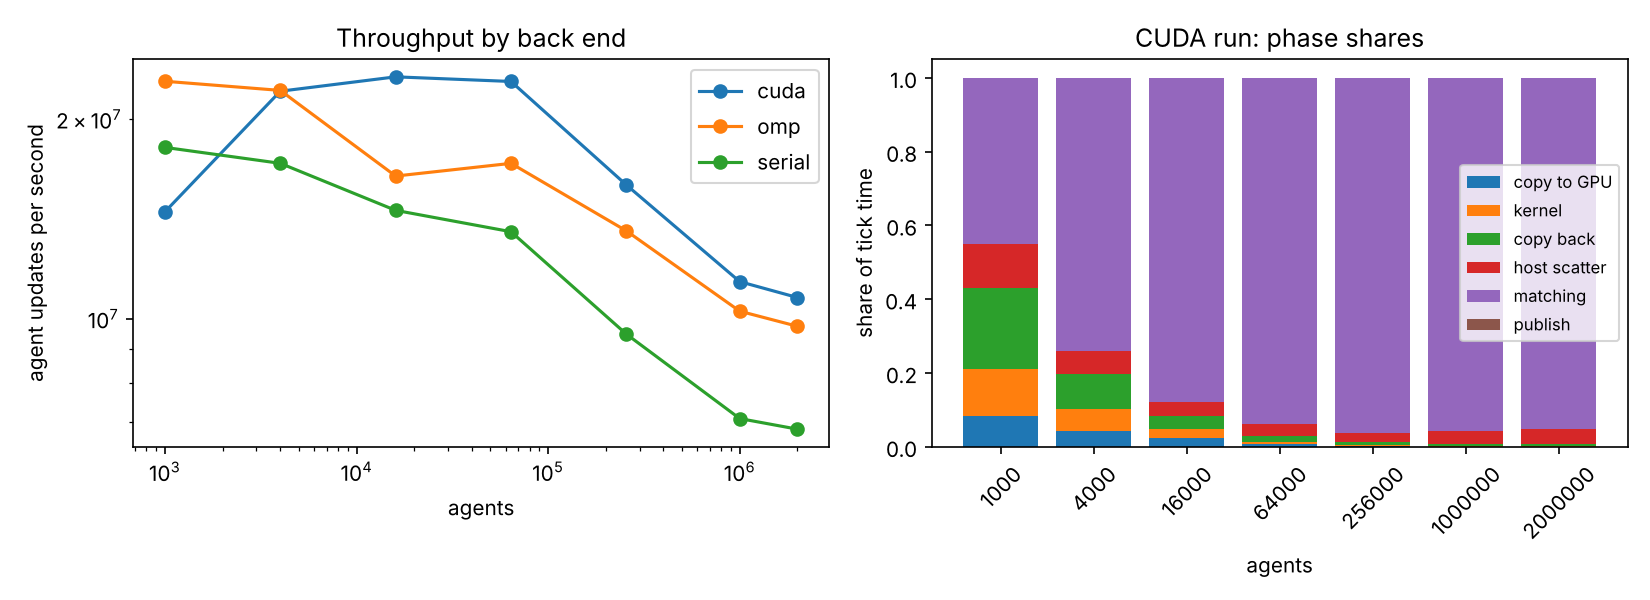
\includegraphics[width=\textwidth]{crossover.png}
\caption{CPU vs GPU crossover on the T4. Left: throughput (agent updates per second) of each back
end. Right: share of tick time per phase in the CUDA runs; matching dominates beyond 16k agents.}
\label{fig:crossover}
\end{widefigure}

Table~\ref{tab:kernel} and Fig.~\ref{fig:cuda} summarise the kernel experiments. Sorting agents by
strategy raises the number of active threads per warp instruction from 16.7 to 22.8 (32 means no
divergence), a 27\% reduction in divergence, and makes the kernel about 7\% faster. Compacting the
copy back to only the agents that acted cuts it from 1.90 to 0.46\,ms per tick (4.1$\times$). Block
sizes from 64 to 256 threads perform within 0.06\,ms of each other; 128 is best.

\begin{table}[t]
\centering
\caption{CUDA kernel metrics (Nsight Compute, 1M agents).}
\label{tab:kernel}
\footnotesize
\begin{tabular}{@{}lrr@{}}
\toprule
Metric & Sorted & Unsorted\\
\midrule
Active threads per warp instr. (of 32) & \textbf{22.8} & 16.7\\
Kernel duration & \textbf{0.138 ms} & 0.149 ms\\
Achieved occupancy & 82\% & 85\%\\
Registers per thread & 27 & 27\\
DRAM bandwidth & 173 GB/s & 168 GB/s\\
\midrule
Copy back, full / compacted & \multicolumn{2}{c}{1.90 ms / 0.46 ms}\\
\bottomrule
\end{tabular}
\end{table}

\begin{widefigure}
\centering
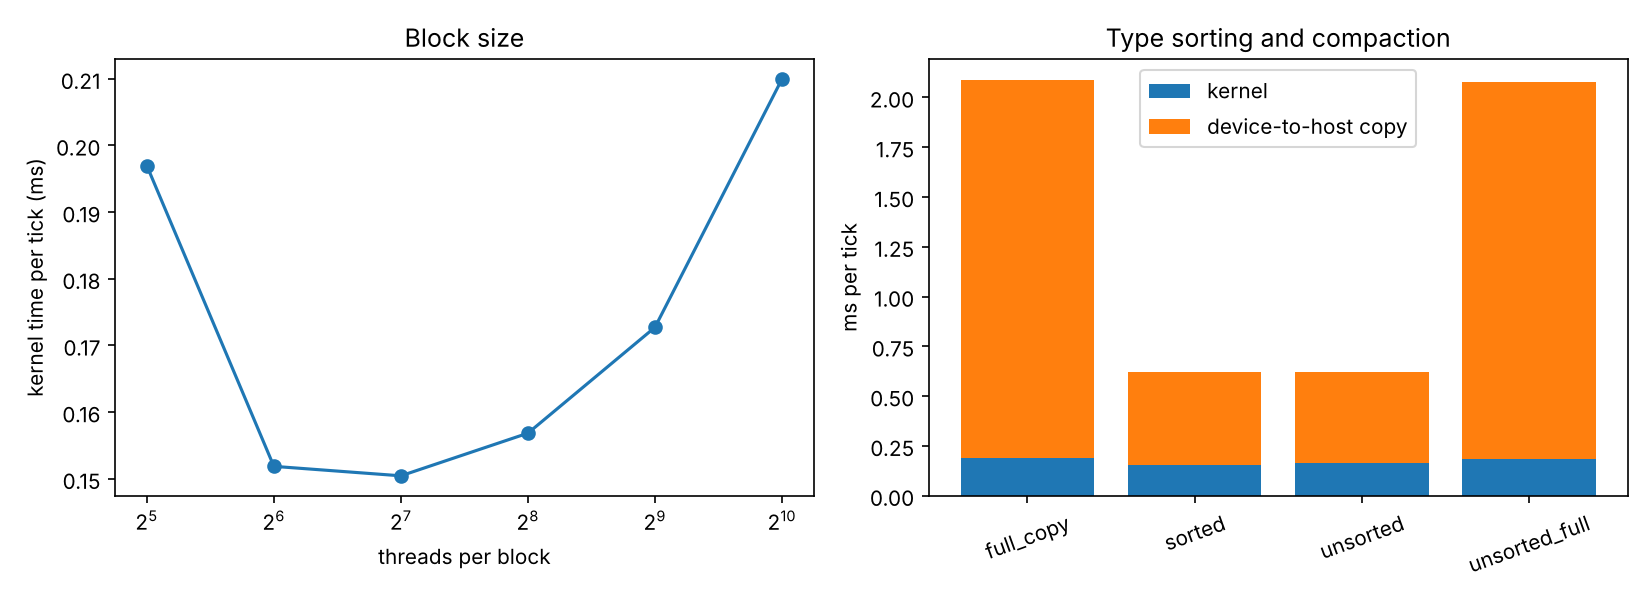
\includegraphics[width=\textwidth]{cuda_experiments.png}
\caption{CUDA kernel experiments. Left: kernel time per tick against block size. Right: kernel and
device-to-host copy time with and without type sorting and compaction.}
\label{fig:cuda}
\end{widefigure}

\subsection{CPU results (16-thread laptop)}\label{sec:res-cpu}
\textbf{Matching across instruments.} Table~\ref{tab:instr} and Fig.~\ref{fig:instr} show the
speedup of OpenMP matching over serial matching as instruments are added, with 16 threads. With one
instrument OpenMP is slightly \emph{slower} (0.90$\times$): there is nothing to split, so the only
effect is overhead. Speedup grows only as instruments are added, reaching 3.97$\times$ at 128.

\begin{table}[t]
\centering
\caption{OpenMP matching speedup over serial vs number of instruments (200k agents, 16 threads).}
\label{tab:instr}
\footnotesize
\setlength{\tabcolsep}{3.5pt}
\begin{tabular}{@{}lrrrrrrrr@{}}
\toprule
Instruments & 1 & 2 & 4 & 8 & 16 & 32 & 64 & 128\\
\midrule
Speedup & 0.90 & 0.97 & 1.97 & 2.14 & 2.63 & 3.23 & 3.54 & \textbf{3.97}\\
\bottomrule
\end{tabular}
\end{table}

\begin{figure}[t]
\centering
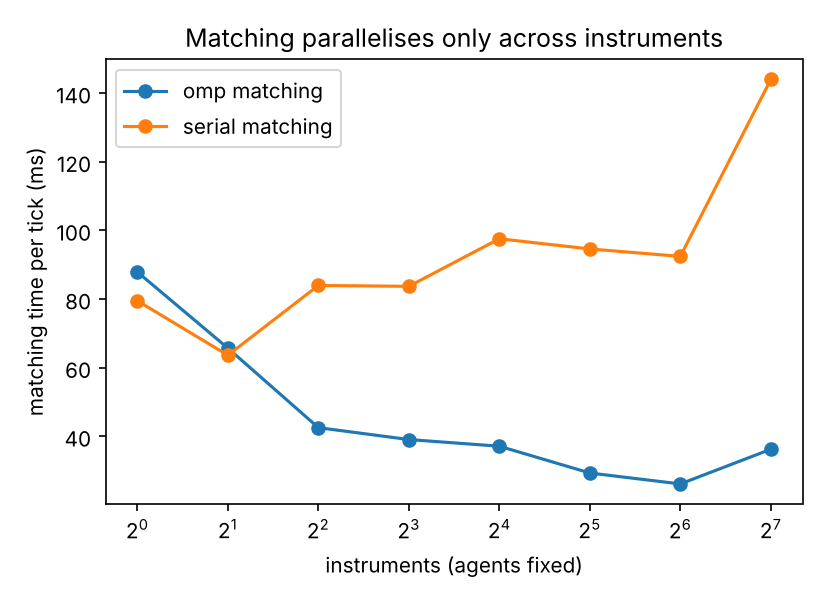
\includegraphics[width=0.85\columnwidth]{instruments.png}
\caption{Matching speedup grows only with the number of instruments.}
\label{fig:instr}
\end{figure}

\textbf{Strong scaling.} Table~\ref{tab:strong} and Fig.~\ref{fig:strong} show the whole simulation
with a fixed problem. Speedup peaks at 1.99$\times$ on 8 threads and falls to 1.74$\times$ on 16.
The decision phase, which needs no coordination between agents, improves only 1.75$\times$ on 8
threads (2.30\,s to 1.31\,s).

\begin{table}[t]
\centering
\caption{Strong scaling (400k agents, 64 instruments, 300 ticks, median of 5).}
\label{tab:strong}
\footnotesize
\setlength{\tabcolsep}{4pt}
\begin{tabular}{@{}lrrrrrr@{}}
\toprule
Threads $p$ & serial & 1 & 2 & 4 & 8 & 16\\
\midrule
Time (s) & 17.4 & 17.2 & 14.3 & 9.8 & 8.7 & 10.0\\
Speedup $S$ & 1.00 & 1.01 & 1.21 & 1.78 & \textbf{1.99} & 1.74\\
Efficiency $E$ & 1.00 & 1.01 & 0.61 & 0.45 & 0.25 & 0.11\\
Karp--Flatt $e$ & -- & -- & 0.65 & 0.42 & 0.43 & 0.55\\
\bottomrule
\end{tabular}
\end{table}

\begin{widefigure}
\centering
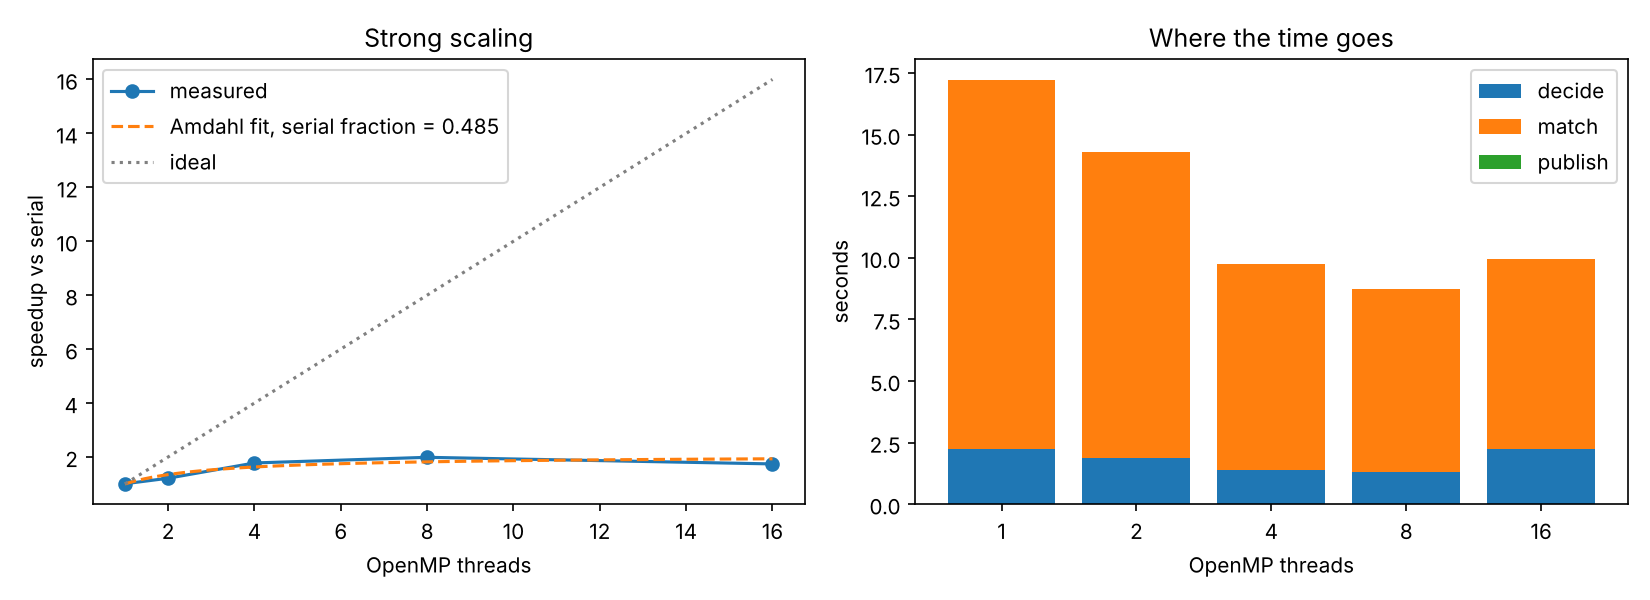
\includegraphics[width=\textwidth]{strong_scaling.png}
\caption{Strong scaling on the laptop. Left: measured speedup, Amdahl fit (serial fraction 0.485)
and ideal. Right: time per phase; matching dominates at every thread count.}
\label{fig:strong}
\end{widefigure}

\textbf{Weak scaling.} With 50{,}000 agents and 8 instruments per thread
(Table~\ref{tab:weak}, Fig.~\ref{fig:weak}), time should stay constant under ideal scaling. Instead,
efficiency falls to 0.11 at 16 threads, and total throughput levels off at about 11 million agent
updates per second, 1.8$\times$ the single-thread rate.

\begin{table}[t]
\centering
\caption{Weak scaling (50k agents and 8 instruments per thread, median of 5).}
\label{tab:weak}
\footnotesize
\begin{tabular}{@{}lrrrrr@{}}
\toprule
Threads & 1 & 2 & 4 & 8 & 16\\
\midrule
Time (s) & 2.40 & 3.62 & 6.27 & 11.07 & 21.85\\
Efficiency & 1.00 & 0.69 & 0.40 & 0.22 & 0.11\\
Updates/s (M) & 6.3 & 8.3 & 9.6 & 10.8 & 11.0\\
\bottomrule
\end{tabular}
\end{table}

\begin{figure}[t]
\centering
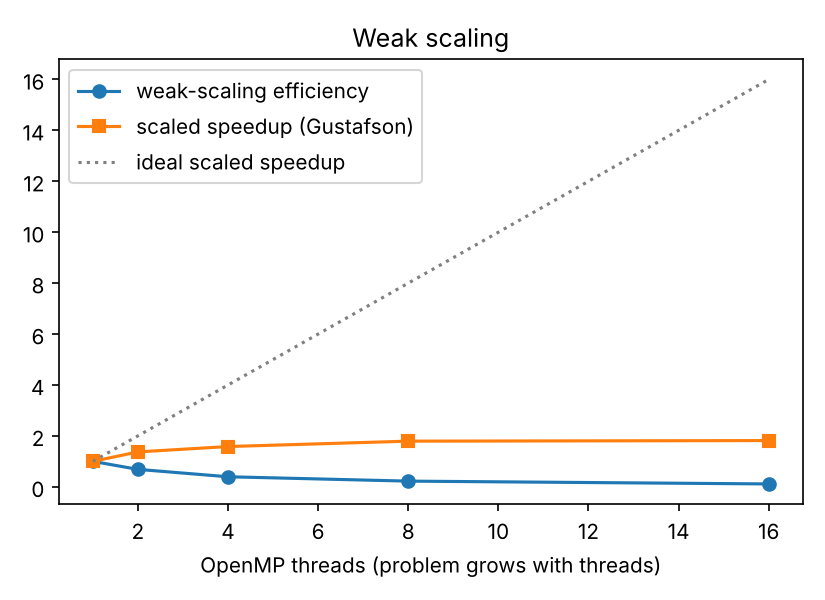
\includegraphics[width=0.85\columnwidth]{weak_scaling.png}
\caption{Weak scaling efficiency on the laptop.}
\label{fig:weak}
\end{figure}

\textbf{MPI.} With 400{,}000 agents and 64 instruments split over 1, 2 and 4 ranks on the same
machine (Fig.~\ref{fig:mpi}), communication plus waiting at the per-tick barrier takes 0\%, 20\%
and 39\% of tick time respectively. The message itself is one 64-bit integer; almost all of this
time is ranks waiting for the slowest rank, so it measures load imbalance more than message cost.
Total time barely changes, because the ranks share the same cores.

\begin{figure}[t]
\centering
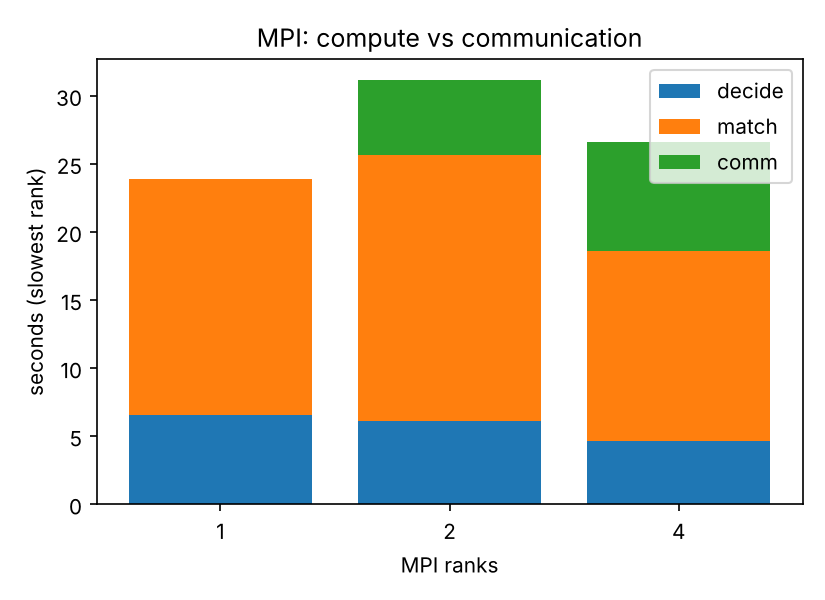
\includegraphics[width=0.85\columnwidth]{mpi.png}
\caption{MPI: share of tick time spent in communication and barrier wait.}
\label{fig:mpi}
\end{figure}

\textbf{False sharing.} With per-thread counters padded to separate cache lines, matching took
22.0\,ms per tick; unpadded, 20.8\,ms. The difference is within run-to-run noise: each thread
updates the counters only a few times per instrument per tick, so cache-line contention is too rare
to show. We report this as a negative result.

\subsection{Model realism}\label{sec:res-facts}
Table~\ref{tab:facts} and Fig.~\ref{fig:facts} compare the simulated returns with the stylised facts
of real markets~\cite{cont2001}. The model reproduces heavy tails and volatility clustering. It
fails the absence of linear autocorrelation: prices partly bounce back after a move (lag-1
autocorrelation $-0.33$), an effect of the mean-reverting and market-making agents.

\begin{table}[t]
\centering
\caption{Stylised facts of simulated 10-tick returns (16 instruments, 20k ticks).}
\label{tab:facts}
\footnotesize
\begin{tabularx}{\columnwidth}{@{}X r c@{}}
\toprule
Property (real markets) & Measured & Pass\\
\midrule
Heavy tails (excess kurtosis $> 0$) & 4.26 & yes\\
Volatility clustering ($|r|$ ACF lag 1 / lag 10 $> 0$) & 0.20 / 0.09 & yes\\
No linear autocorrelation (ACF lag 1 $\approx 0$) & $-0.33$ & no\\
Hill tail index (real: about 3--5) & 8.0 & partly\\
\bottomrule
\end{tabularx}
\end{table}

\begin{widefigure}
\centering
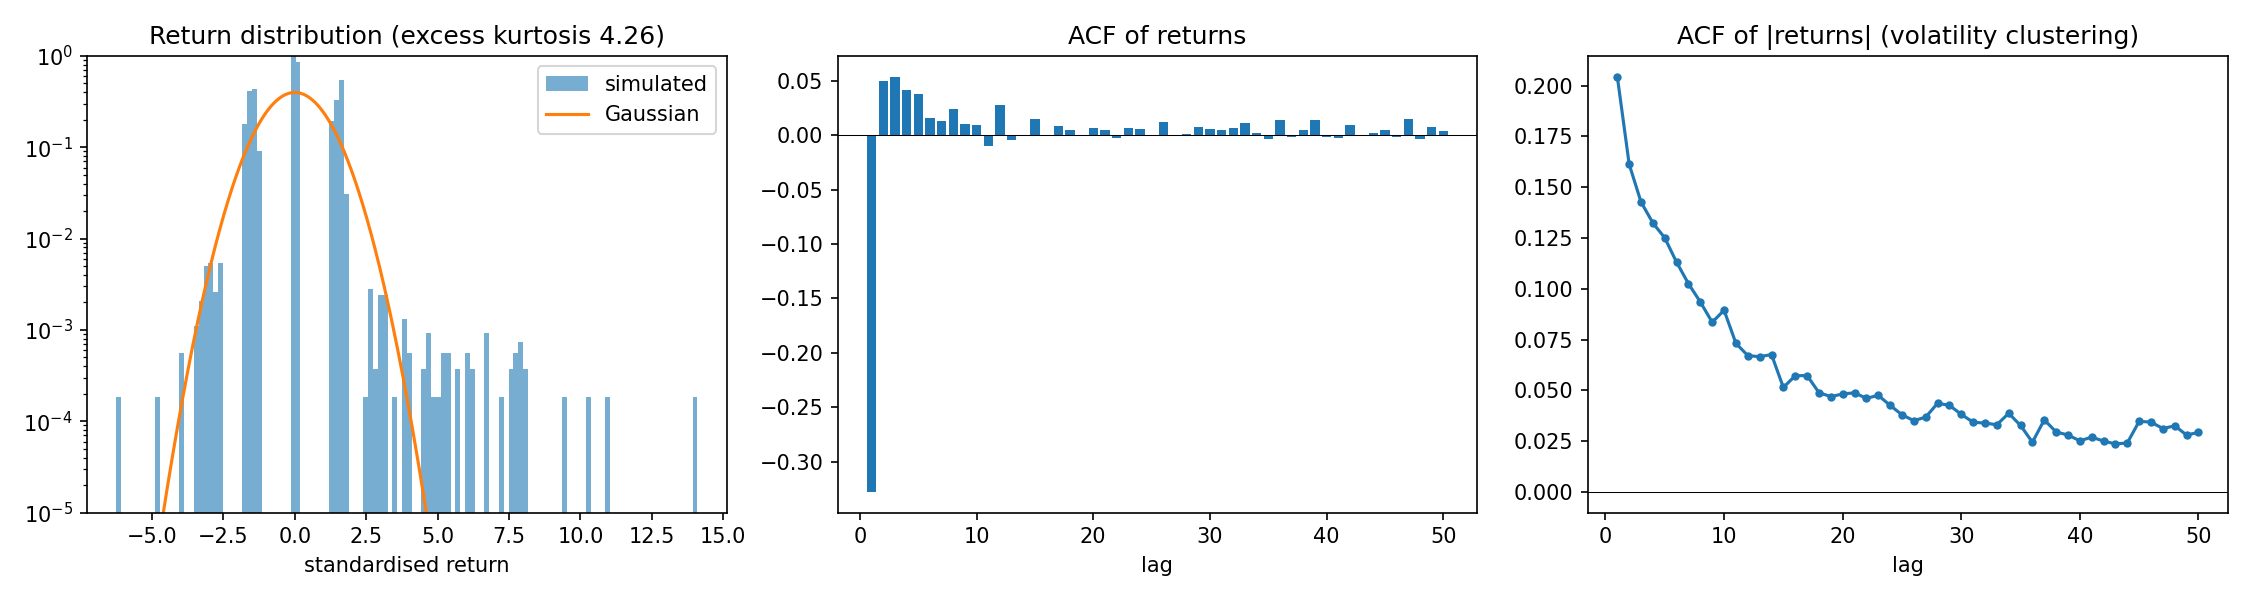
\includegraphics[width=\textwidth]{stylized_facts.png}
\caption{Stylised facts of simulated returns: return distribution against a Gaussian,
autocorrelation of returns and of absolute returns.}
\label{fig:facts}
\end{widefigure}

\section{Performance Analysis}\label{sec:perf}

\subsection{Speedup and efficiency}
Table~\ref{tab:speedups} collects the speedups. The pattern is the same everywhere: the parts that
are parallel over agents speed up well (85$\times$ for the kernel), while anything that includes
matching is limited to between 1.1$\times$ and 4$\times$. Parallel efficiency is high only at low
thread counts: 0.61 at 2 threads and 0.25 at 8 threads in strong scaling.

\begin{table}[t]
\centering
\caption{Summary of speedups.}
\label{tab:speedups}
\footnotesize
\begin{tabularx}{\columnwidth}{@{}X r@{}}
\toprule
Comparison & Speedup\\
\midrule
CUDA kernel vs 2-thread OpenMP decisions (1M agents) & 85$\times$\\
CUDA decision phase incl.\ copies and scatter & 3.6$\times$\\
Copy back, compacted vs full & 4.1$\times$\\
Kernel, type-sorted vs unsorted & 1.07$\times$\\
CUDA tick vs OpenMP tick (best, 16k agents) & 1.41$\times$\\
CUDA tick vs serial tick (32k--2M agents) & 1.54--1.61$\times$\\
OpenMP matching, 128 vs 1 instrument (16 threads) & 3.97$\times$ vs 0.90$\times$\\
Whole simulation, 8 threads (strong scaling) & 1.99$\times$\\
Demo run, 4-core machine: OpenMP / MPI (2 ranks) & 3.40$\times$ / 3.59$\times$\\
\bottomrule
\end{tabularx}
\end{table}

\subsection{Amdahl's law: where the bound comes from}
On the T4, the decision phase is 14\% of the OpenMP tick at 1M agents. Even an infinitely fast GPU
could then give at most $1/(1-0.14) \approx 1.16\times$; we measure 1.11$\times$, close to that
bound. The GPU has made decisions almost free, and matching is 92--96\% of every CUDA tick
(Fig.~\ref{fig:gustafson}). This is the Amdahl bound predicted in the synopsis: matching inside one
instrument is serial, and no GPU can remove it.

On the laptop, fitting Amdahl's law to the strong-scaling speedups gives an effective serial
fraction of $f=0.49$, which caps speedup at about $1/f \approx 2.1\times$. The Karp--Flatt values
(0.42--0.65) are of the same size and do not fall with $p$, so the limit is not simple parallel
overhead. The code's own serial work (publishing the index) takes about 0.001\,s of 17\,s, far too
little to explain $f$. Since even the coordination-free decision phase improves only 1.75$\times$
on 8 threads, we infer that the laptop's shared resources set the limit: a power-limited mobile
CPU lowers each core's clock as more cores become busy, and all cores share one memory bus, to
which matching (hash lookups and pointer chasing) is especially sensitive. This interpretation is
inferred from the timing pattern, not measured with hardware counters. The fitted $f$ is therefore
best read as an \emph{effective} serial fraction: serial code plus hardware saturation.

\subsection{Gustafson's law}
Gustafson's law predicts that growing the problem with the machine keeps efficiency high. On the
T4, growing agents at 32 fixed instruments keeps the CUDA speedup over serial at 1.54--1.61$\times$
from 32k to 2M agents (Fig.~\ref{fig:gustafson}): the speedup does not grow, because more agents
also mean more orders to match. On the laptop, weak-scaling efficiency drops to 0.11 at 16 threads
and throughput levels off at 1.8$\times$ the single-thread rate. Gustafson's law assumes that the
parallel part keeps scaling with more cores; that only holds while memory bandwidth and the power
budget also grow.

\begin{figure}[t]
\centering
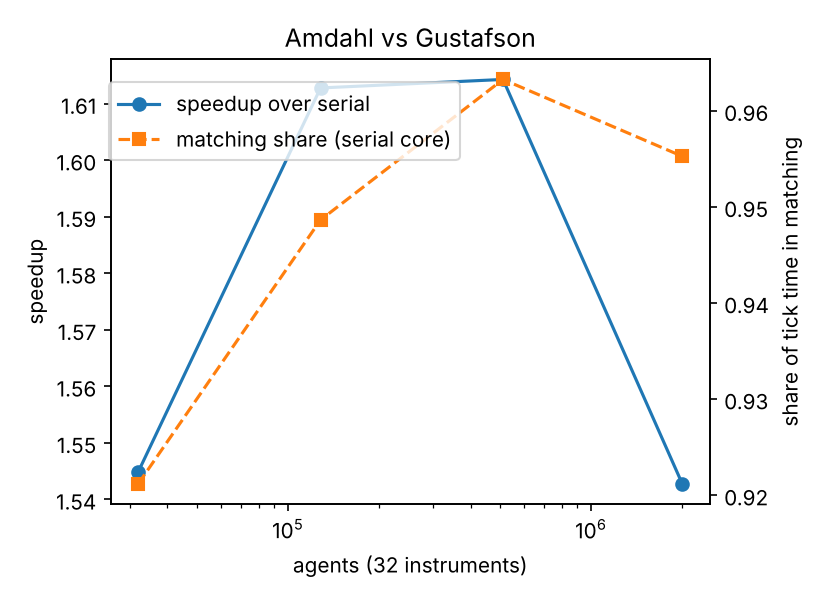
\includegraphics[width=0.85\columnwidth]{gustafson.png}
\caption{Growing agents at 32 fixed instruments on the T4: CUDA speedup over serial and matching
share of tick time.}
\label{fig:gustafson}
\end{figure}

\subsection{Roofline}
The decision kernel performs 3.95 integer operations per byte of DRAM traffic, below the T4's
ridge point of 12.7 (4.07\,Tops/s peak over 320\,GB/s), so it is memory-bound
(Fig.~\ref{fig:roofline}). It reaches 173\,GB/s, 54\% of peak bandwidth, at 82\% occupancy with 27
registers per thread. Further kernel tuning could at most halve a phase that is already under 1\% of
tick time, so it would not change the end-to-end result.

\begin{figure}[t]
\centering
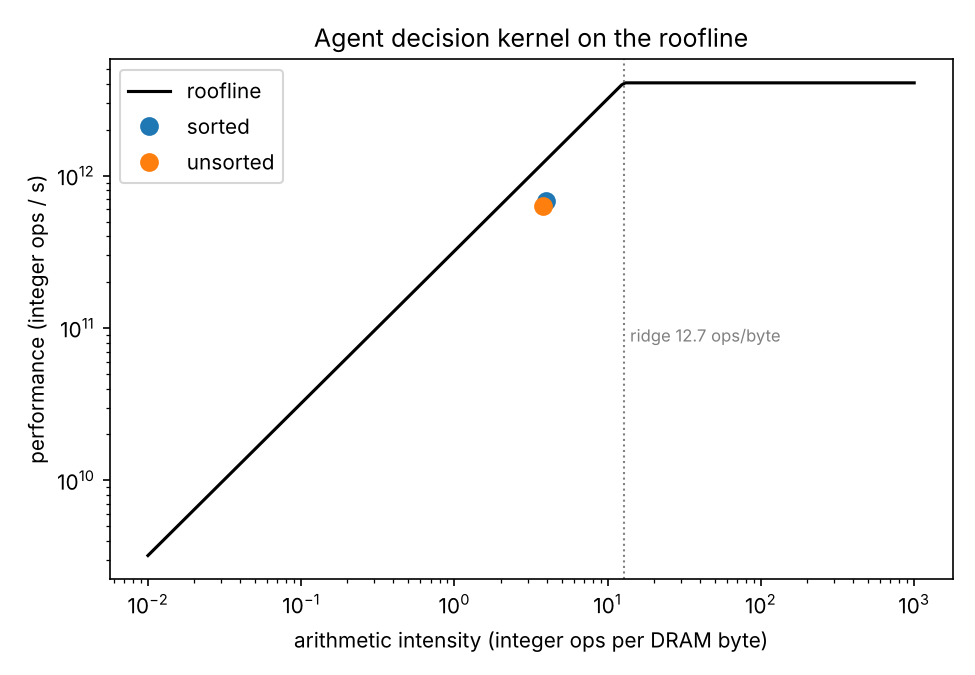
\includegraphics[width=0.85\columnwidth]{roofline.png}
\caption{Roofline placement of the decision kernel on the Tesla T4 (integer operations).}
\label{fig:roofline}
\end{figure}

\subsection{CPU vs GPU threshold}
Heterogeneous execution beats the multicore CPU when the GPU's saving on decisions exceeds the
fixed cost of the CPU--GPU boundary (two copies, a launch and the host scatter). On the T4 this
happens between 4{,}000 and 16{,}000 agents. The advantage then shrinks with size, because the
matching time that the GPU cannot touch grows with the number of orders. The threshold also depends
on the CPU: with more CPU threads, OpenMP decisions are faster, so the GPU needs more agents to pay
off. Finally, the host scatter (about 3.2\,ms at 1M agents) costs 20 times the kernel; moving more
of the pipeline to the GPU would only pay if matching moved too, which price--time priority
prevents within an instrument.

\subsection{Bottleneck summary}
\begin{itemize}
\item \textbf{Matching} under price--time priority is the bottleneck on every back end: 92--96\% of
  a CUDA tick, and it parallelises only across instruments.
\item \textbf{The CPU--GPU boundary} (copies and host scatter) costs more than the kernel; compaction
  reduces it by 4.1$\times$.
\item \textbf{Hardware saturation} (power and memory bandwidth) limits CPU scaling to about
  2$\times$ on the laptop before the code's own serial part does.
\item \textbf{MPI} cost is dominated by load imbalance at the per-tick barrier, not by data volume.
\end{itemize}
